\documentclass{article}
\usepackage{fasy-hw}

\author{Joshua Harthan}
\problem{1}
\begin{document}
Suppose you have a map that consists of six vertical strips.
So, each region has two neighbors: one left and one right (except the leftmost region does not have a left neighbor and the rightmost region does not have a right neighbor). If we have five possible colors, and paint each region randomly, with equal probability of each color:
\item[]1.1 What is the probability that the coloring is a four-coloring?
\item[]1.2 What is the expected number of colors that you will use?
\item[]1.1 The probability that the coloring is a four-coloring is equivalent to the total number of ways to color the map with four colors divided by the total number of ways to color the map with five colors. To get both of these numbers, we can put this into the equation P(4) = $4 \times 3 \times 2^{2}$ = 48 and P(5) =  $5 \times 4 \times 3^{2}$ = 180. Therefore the probability of the map being a four coloring is equivalent to $\frac{48}{180}$ = $\frac{4}{15}$ = .267.
\item[]1.2 The maximum expected number of colors that is to be used is two as the countries won't have touching, repeated colors due to the countries only having two neighbors(except for the outer two countries). Since this is true, the maximum amount of colors needed to color the map is only two.

\problem{2}
\collab{none}
\clearpage
\header
9.1 Question 20
\item[]Suppose you are appearing on a game show with a prize behind one of five closed doors: $A, B, C, D,$ and $E$. If you pick the right door, you win the prize. You pick door A. The game show host then opens one of the other doors and reveals that there is no prize behind it. Then the host gives you the option of staying with your original choice of door $A$ or switching to one of the other doors that is still closed.
\item[]a. If you stick with your original choice, what is the probability that you will win the prize?
\item[]b. If you switch to another door, what is the probability that you will win the prize?
\item[]a. The probability that the prize is behind the door you chose P($A$) is equivalent to $\frac{1}{5}$ as there are five possible doors and the probability that you chose the correct door on the first pick is 1 out of 5.
\item[]b. If you switch to another door, and another door that doesn't have a prize behind it is opened, the probability of winning a prize is $\frac{4}{15}$. This is because the probability of the other four doors having a prize behind them is $\frac{4}{5}$, due to the probability of you choosing the door is $\frac{1}{5}$, i.e. 1 - P$(A)$ = 1 - $\frac{1}{5} = \frac{4}{5}$. Since you have to choose between three doors, when given the opportunity to switch, as one is already opened that doesn't contain a prize, the probability of the doors containing the prize are all equivalent to $\frac{1}{3}$, let's call this probability P($B$). So given these probabilities, you multiply the two together to get P$(A|B)$ = $\frac{4}{15}$.


\problem{3}
\collab{none}
\clearpage
\header
9.2 Question 7
\item[]One urn contains one blue ball (labeled $B_1$) and three red balls (labeled $R_1, R_2,$ and $R_3$). A second urn contains two red balls ($R_4$ and $R_5$) and two blue balls ($B_2$ and $B_3$). An experiment is performed in which one of the two urns is chosen at random and then two balls are randomly chosen from it, one after the other without replacement.
\item[]a. Construct the possibility tree showing all possible outcomes of this experiment.
\item[]b. What is the total number of outcomes of this experiment?
\item[]c. What is the probability that two red balls are chosen?
\item[]a. \begin{figure}[h!]
  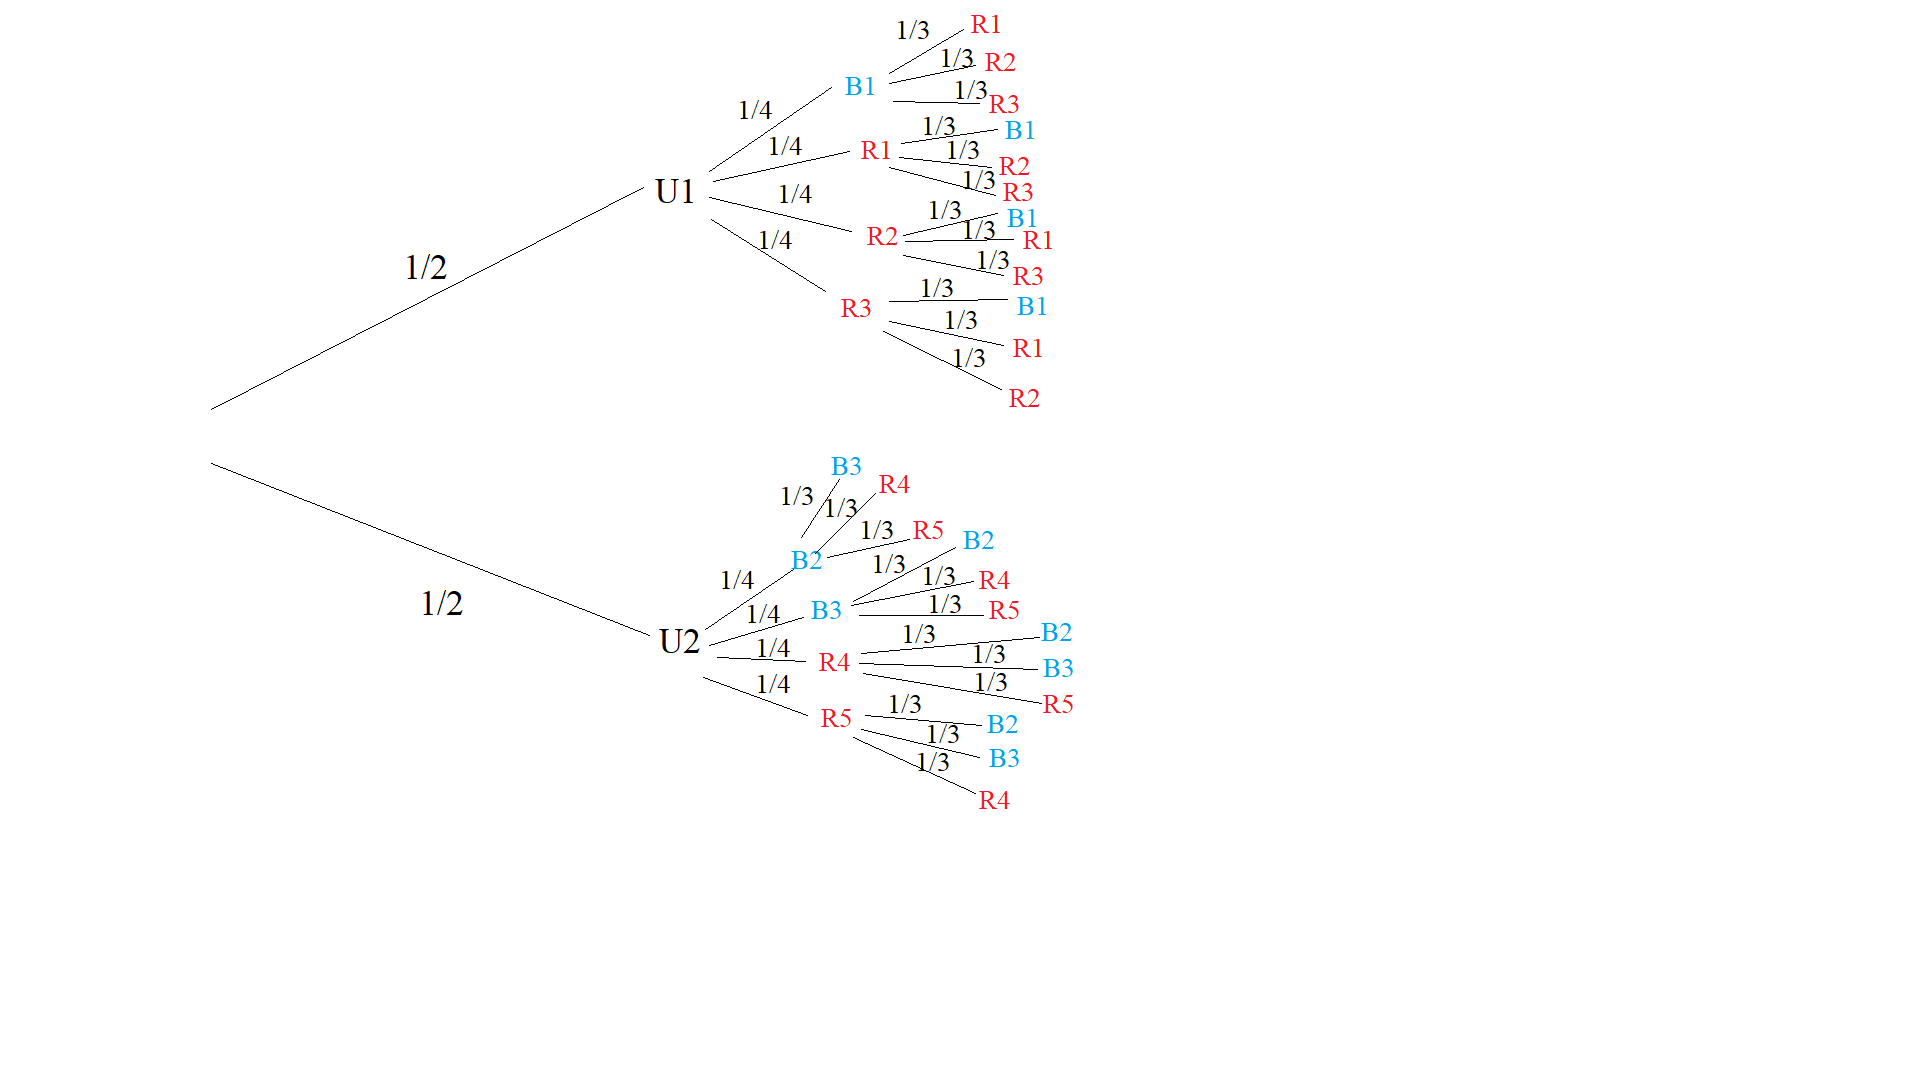
\includegraphics[width=\linewidth]{Untitled.png}
  \caption{Possibility Tree}
  \label{fig:map1}
\end{figure}
\clearpage
\header
\item[]b. The total number of outcomes from this experiment is $2 \times 4 \times 3$ = 24 different outcomes.
\item[]c. The probability that two red balls are chosen is the probability $\frac{8}{24}$ = $\frac{1}{3}$. This is due to the fact that out of the twenty-four possible outcomes, eight are choosing two red balls out of the two urns.

\problem{4}
\collab{none}
\clearpage
\header
9.3 Question 16
\item[]a. How many strings of four hexadecimal digits do not have any repeated digits?
\item[]b. How many strings of four hexadecimal digits have at least one repeated digit?
\item[]c. What is the probability that a randomly chosen string of four hexadecimal digits has at least one repeated digit?
\item[]a. Since there are 16 different digits for the hexadecimal system, the number of possibilities of non repeated digits are $16 \times 15 \times 14 \times 13$ = 43,680 as there are 16 possibilities of a digit for the the first number in the string, 15 possibilities for the second, 14 possibilities for the third, and 13 possibilities for the fourth.
\item[]b. The total number of strings with four hexadecimal digits is equivalent to $16^{4}$ = 65,536 different possibilities. Since we already calculated the number of strings that do not have any repeated digits, and we are only looking for strings that have at least one repeated digit, we can subtract the total from this calculated value. Therefore we get 65,536 - 43,680 = 21,856 strings of four hexadecimal digits that have at least one repeated digit.
\item[]c. The probability that a randomly chosen string of four hexadecimal digits has at least one repeated digit is equivalent to the number of at least one digit repeated divided by the total number of strings which is equivalent to $\frac{21,856}{65,536}$ = .333496.


\problem{5}
\collab{none}
\clearpage
\header
Hedy Lamarr was an American film actress and self-taught inventor known for, along with George Antheil, developing a radio guidance system meant for the usage of Allied torpedoes to jam Axis technology during World War II. Despite not being used by the military until the 1960s, this technology formed the basis of technology used in both Bluetooth and early versions of Wi-Fi. Both bluetooth and wi-fi are important to the field of computing in that both of these systems are widely used to connect seamlessly to the other devices and the internet today, and without such technology computers would have to rely heavily on being connected with wires and therefore not be portable. Without Hedy Lamarr developing the groundwork for such technologies, we would not be able to afford such luxuries as laptops or even mobile phones.  
\item[]\url{https://en.wikipedia.org/wiki/Hedy_Lamarr}

\end{document}